\documentclass[UTF8,12pt]{ctexbook}
\usepackage{graphicx}
\usepackage{float}
\title{\textbf{THE HISTORY}}
\author{}
\date{}
\begin{document}
\maketitle
\tableofcontents
\chapter{简介}
    \section{总述}
    \section{Yealsor}
        \subsection{Yealsor的地理}
        Yealsor主要由Silder平原、Queto平原、
        Funo丘陵、Viruna和Finua高原构成。
        其中有三条主要的河流,
        分别为Pukral、Amiso和Kaludin,
        最主要的是Pukral和其支流Amiso,
        它们诞生并哺育了Lmids文明、Aeray文明和古王朝文明。

        Pukral发源于Finua高原,
        Amiso则发源于Finua高原东部的Turzen山脚,
        二者穿过Funo丘陵交汇于Queto平原,
        随后穿过Erosa山脉抵达Slider平原并流入海洋。

        Finua高原西北部是Viruna山地,
        Kaludin发源于此,
        穿过Hulin丘陵、Euro平原和Yotin丘陵并流入大海。
        相较于Pukral和Amiso,
        Kaludin经过的平原地区很少,
        因此这条河流周围仅仅只有少量的聚落,
        并没有独立发展出文明。
        
        Yealsor地区位于高压带上,
        季节性降水明显,
        又由于Erosa山脉的阻挡,
        Queto平原东西两面气候类型不尽相同,
        西部的Euro平原由于地势低洼,
        夏季能获得充沛的降水,
        容易形成大面积沼泽,
        而东部的Aptone平原因为Erosa山脉挡住了季风带来的雨水,
        因此较为干旱,
        表现为草原气候。

        北部的Silder平原表现为热带季风气候,
        但不规则的降水往往会导致洪涝灾害的发生,
        不同于Queto平原拥有众多湖泊和沼泽能够囤积雨水以渡过冬季的干旱,
        Slider平原的洪涝和干旱的灾难频发,
        因此虽然拥有充足的降水和资源,
        但文明远没有Queto平原安逸。
        \subsection{Yealsor的景观特点}


        \newpage
        \begin{figure}[!h]
            \centering
            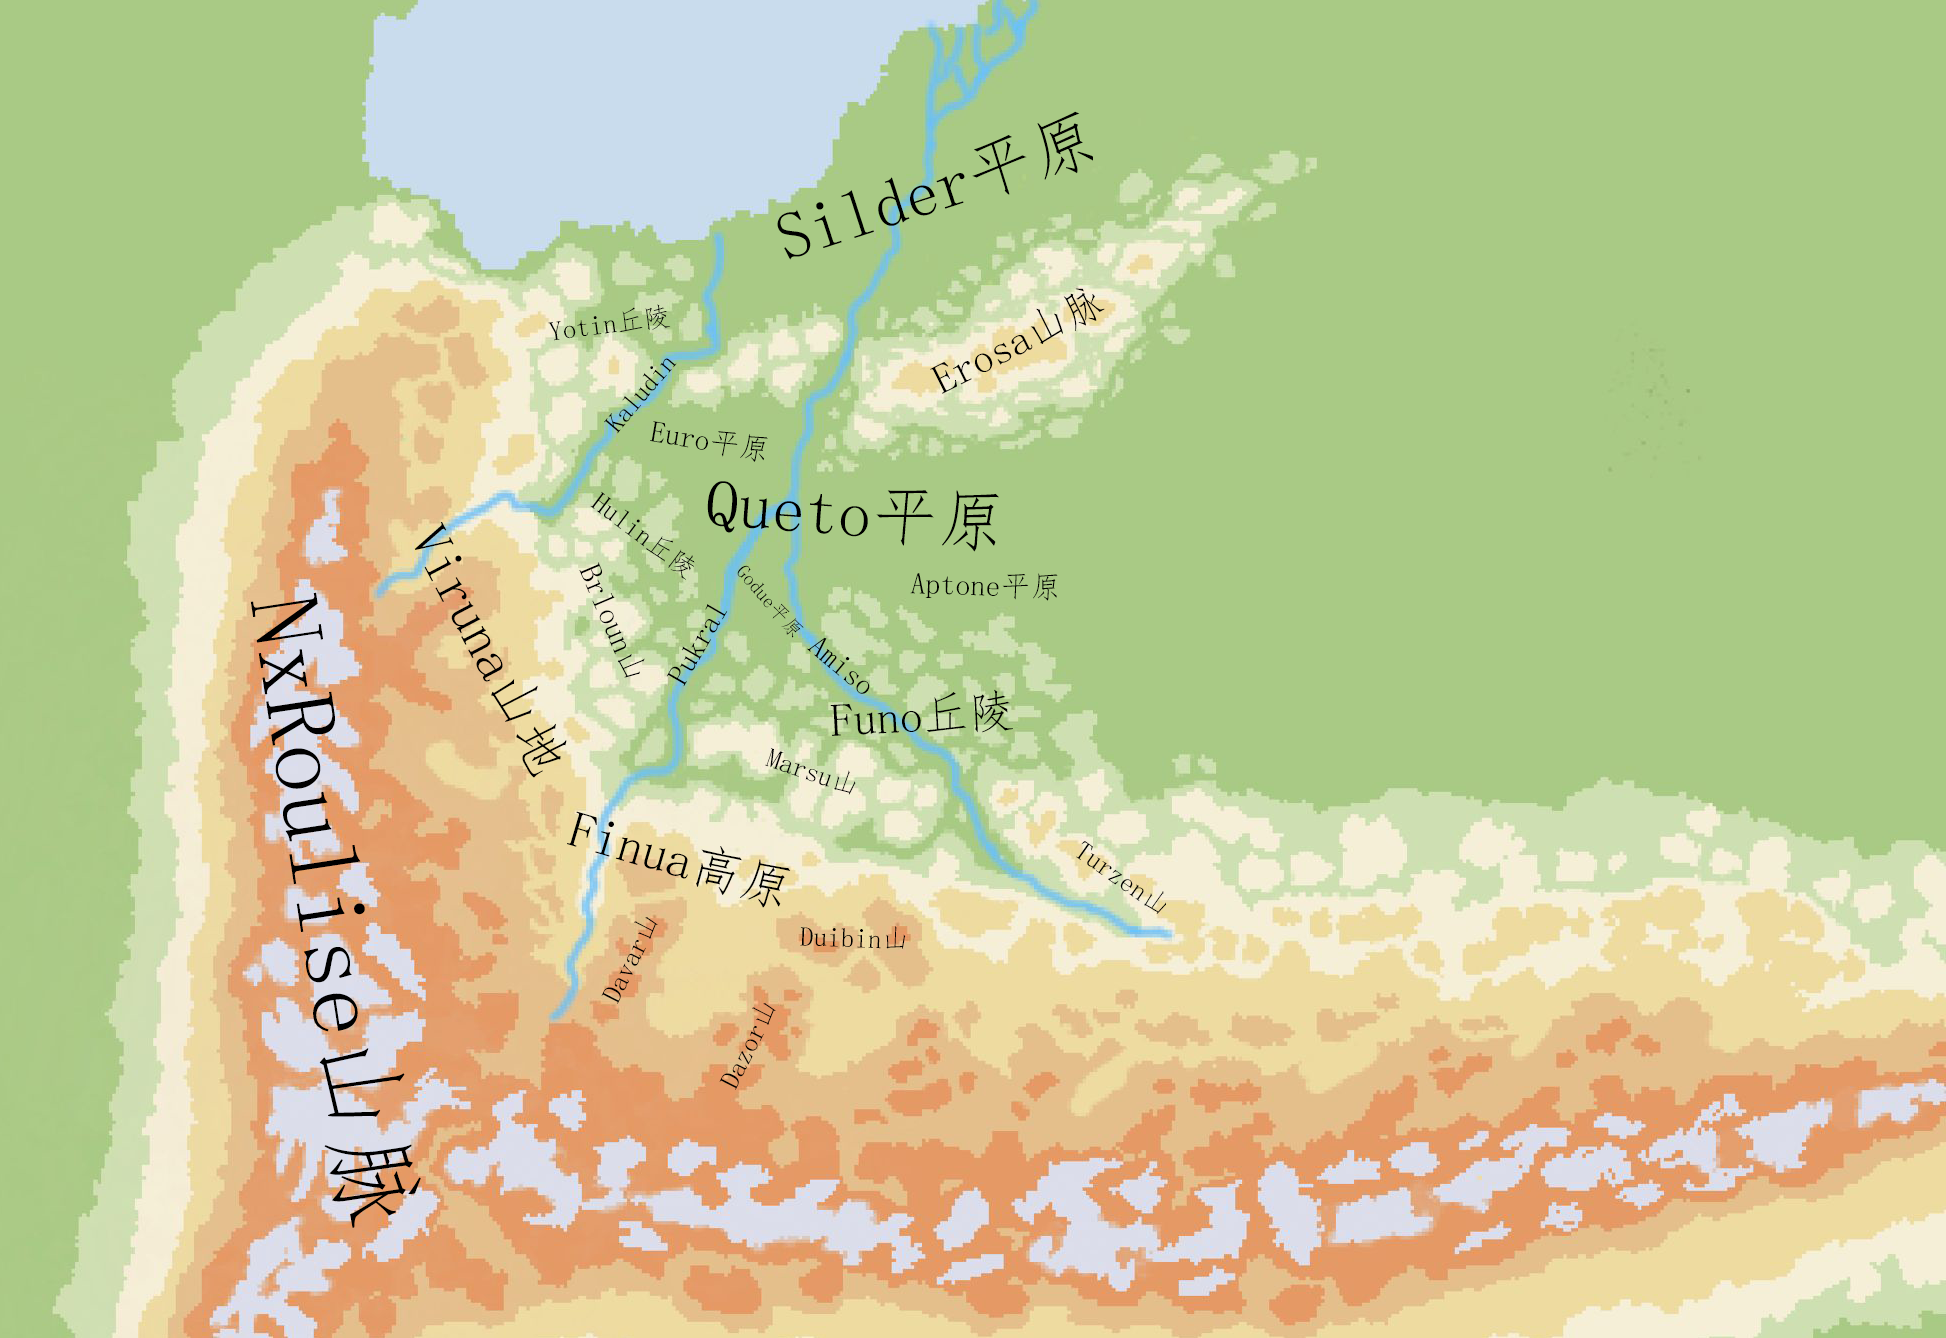
\includegraphics[scale=0.2]{Yealsor.png}
            \caption{Yealsor地图}
        \end{figure}
        

        

\part{Yealsor史}
    \chapter{Yealsor早纪史}
    得益于Queto平原的独特优势,
    Lmidure人在前LC100年左右进入了青铜器时代,
    各大城邦逐渐被建立起来,
    并大肆去周边部落掠夺奴隶,
    许多部落因此只能沿着河流上流,
    抵达Funo丘陵和Finua高原生活,
    从此,
    Lmidure人分成了两支,
    依然居住在Queto平原的Lmids人和生活在南部山区的Aeray人。
        \section{僭主、民主与共和}
            Lmids文明的城邦政治是Yealsor文明政治体系的源头,
            在他们的探索下,
            诞生其独特的民主、君主和贵族政治。
            由于城邦分散的特性,
            三种不同的政治体系在各个城邦独立发展,
            其中在民主制城邦体系下最早提出了法政原则,
            提出了第一部成文法,
            同时也编撰了第一部法典。

            而君主政体的城邦则提出了民本君主制,
            有效化解了君主和平民之间的矛盾,
            为后世封建君主提供了典范,
            配合君主制的还有一套极其高效的官僚制度,
            在Lurte王国的统治时,
            君主制和民主制的融合的过程中也产生了权力分立的思想,
            这不仅仅影响了整个Yealsor文明,
            甚至在被殖民征服的世界反向到了西方的世界,
            为那里带来了巨大的变革。
            \subsection{僭主到君主的转变}
                Lmdis文明的君主制以Xiuna城邦的君主制为代表,
                Xiuna是Euro地区的一座城邦,
                它兴起于前LC63年,
                坐落于Garlum沼泽,
                以手工业和农业为基础,
                大量吸收了周围部落人口,
                是当时较为繁荣的城邦之一。

                随着人口的增加,
                Xiuna城邦内部的矛盾不断激增,
                最为代表的是自由民和公民之间的矛盾。
                繁荣的经济吸引了大量的自由民的加入,
                他们农忙时在城外耕作,
                农闲时则进入城邦从事手工业生产。
                这些自由民居住在城邦内脏乱的地方,
                他们大多数人并没有固定的居所,
                被当地人视为流贼百般提防。

                前LC38年中冬季,
                饥荒蔓延,
                公民尚不能果腹,
                更不用说被视为流贼的自由民了,
                他们为了生存,
                只能通过偷窃和乞讨的方式获得一点食物。
                可越来越多的偷窃事件发生,
                不仅没有解决自由民的困境,
                反而让那些清白的人背上了莫须有的偏见甚至罪名。

                前LC38年中冬季7月,
                一些公民兵出于一己私利,
                借以抓窃贼的名义冲入贫民区,
                对当地的自由民肆意的掠夺和拘捕,
                夺走了那些他们本就所剩无几的财产。
                这一行为引起了自由民的不安,
                随后便激起了不满,
                暴动随之发生。
                \subsubsection{篡夺者\emph{Ielous}}
                元老院指派Farane家族的\emph{Ielous}进行镇压,
                公民兵很快封锁了街区,
                一天之内便平息了暴动,
                拘捕并当场处决了大量的暴乱人群。
                但是这只是表面上的,
                待夜晚降临,
                暗杀事件四处发生,
                大量自由民从街巷中涌出,
                夺取了位于城郊的武器库。

                暴动演变为了一场战争,
                \emph{Ielous}面对的不再是手无寸铁的平民,
                而是具有武装且极度愤怒的士兵,
                为了避免冲突的扩大,
                \emph{Ielous}私下和暴民们进行了谈判,
                当即处决了那些肆意闯入贫民区的公民兵和一些负责镇压的将领。
                \emph{Ielous}先斩后奏的行为让元老院很不满,
                可就在元老贵族们对\emph{Ielous}进行声讨的时候,
                \emph{Ielous}统御的公民兵和收编的自由民闯入并强行解散了元老院。
                
                架空了元老院的\emph{Ielous}在之后履行了他的承诺,
                赋予了大量自由民公民身份,
                并且扩大了元老院的规模,
                修建了广厅元老院。
                元老院成员不再局限于贵族,
                城邦内部所有成员都有机会参与其中。
                虽然\emph{Ielous}扩大了元老院的规模,
                但是他并没有剥夺原来元老院成员的身份,
                因此即使有新的势力加入,
                贵族依然强盛,
                只是屈服于\emph{Ielous}的权威,
                他们并没有展现出自己的敌意。
                \subsubsection{葬仪之乱}
                这种微妙的关系持续到\emph{Ielous}的逝去,
                前LC30年早夏季,
                \emph{Ielous}病逝,
                广厅元老院一致同意为其举办一场隆重的葬礼,
                表面上都在商量葬礼的安排,
                可背后却暗流涌动,
                青年贵族组织并拉拢了传统军官,
                准备在葬礼中夺取\emph{Ielous}的棺椁并恢复旧元老院制度。

                获得了元老身份的自由民不会愿意放弃他们的权力,
                但即使他们秘密得知了青年贵族们的计划也并不能直接展开行动,
                \emph{Ielous}的逝去让旧贵族重新站了起来,
                贸然行动只会激起冲突,
                可失去了\emph{Ielous}的保障,
                冲突的结果只会是贵族们的胜利。

                双方都在秘密地筹划着,
                各自想尽办法拉拢军官,
                排除异己。
                最终在葬仪上双方爆发了冲突,
                或许这边是篡夺者应有的报应,
                他死后也不得安宁,
                厮杀的吼声、飞溅的血液和散乱的肢体分散在他的棺椁旁,
                城邦毫无疑问陷入了内战之中。

                贵族们取得了巨大的优势,
                可令他们没有注意到的是被他们以为除掉的\emph{Magee}出现在了众人面前,
                \emph{Magee}作为\emph{Ielous}之子,
                理应守护父亲的棺椁,
                哪怕是贵族们的士兵,
                此时也不再能阻拦,
                否则便是触怒诸神,
                会得到最严厉的惩罚。

                \emph{Ielous}的葬仪结束,
                青年贵族们失败了,
                参与者全部被捕,
                广厅元老院在一场紧急会议下宣布解散,
                取而代之的是主政团与民政团。
                在对葬仪之乱的参与者逐一审判后,
                大量贵族被处决和流放。
                元老院制度被废除了,
                \emph{Magee}在之后的城邦管理中,
                基于主政团与民政团建立了主政院和民政院,
                两院统称为政院制度,
                是Xiuna君主制的正式开端,
                也是从僭主到君主的根本性改变。

                在Xiuna城邦甚至整个Queto地区里,
                出现过许多类似\emph{Ielous}的独裁者,
                但是他们的统治往往伴随着他们的死亡而结束。
                而Xiuna的两院制度让僭主政治转变为了以官僚政治为基础的君主制政体,
                确保了统治者能够稳定地将权力传到继任者手中。
            \subsection{君主制的发展历程}
                \subsubsection{选举继承制}
                政院制度下,
                主政院由王室成员构成,
                负责掌管城邦的外交、军事和行政等事务,
                而民政院则负责民事相关内容,
                其中包括税务、裁判、调解、建设等相关内容。
                民政院是两院制度的核心,
                在民政院早期,
                成员的任免主要由主政院安排。

                君主制的前提是君主的权力能够平稳地传递到继位者手中,
                而确保这一切的是主政院,
                在主政院内部,
                君王是最高的管理者,
                也是整个城邦的统治者。

                对于君王的任命,
                主政院内部首先采用的是委任制度,
                可随着\emph{Magee}的离世,
                主政院内部产生了矛盾,
                其兄觊觎王位,
                而其子并不愿意让出,
                矛盾导致了宫廷谋杀,
                但这没有结束,
                一场谋杀的出现引发了后续诸多的其他谋杀。

                为了城邦的稳定和自身的安全,
                王室的家族长老一致决定通过主政院内部选举的方式来选举继位者,
                这一制度延续了数十年,
                直到Lukadilous战争后期,
                因为战争议和问题再次导致了宫廷的分裂,
                Xiuna和Lemsa各自为政,
                脱离了主政院的控制。

                而出逃Lurte城邦的王女借着联姻对Xiuna和Lemsa发动了继位者战争,
                取得了战争的胜利后,
                Lurte王室控制了主政院,
                选举继承制被长嗣继承法取代,
                长达半百年的Xiuna王室结束。
                \subsubsection{卫城理政}
                裁决战争后,
                \emph{Kusa}获得了对于Lemsa城邦的实际统治权,
                但主政院不可能同时在Lemsa城邦也设立一个,
                \emph{Kusa}也不希望将Lemsa城邦作为某种附属城邦对待而轻视其管理。
                恰恰相反,
                对于\emph{Kusa}而言,
                Xiuna城邦并非\emph{Kusa}的所有物,
                他只是被主政院和民政院所认可的君主,
                而Lemsa城邦反而是\emph{Kusa}的所有物,
                他是以征服者的姿态去统治这座城邦,
                Lemsa城邦对于\emph{Kusa}而言反而具有更重要的地位。

                主政院不会允许\emph{Kusa}私自将整个Lemsa城邦当作自己的财产处理,
                可碍于君主的身份,
                双方并没有太大的冲突,
                最终达成了妥协。
                在Lemsa城邦和Xiuna城邦中间的一座山丘之上建立卫城作为王宫和新的主政院。
                Xiuna城邦和Lemsa城邦平常则交由民政院管理。
                基于卫城理政的思想,
                王室摆脱了长期的城邦观念,
                王国的概念从中产生,
                Xiuna城邦降级为了一个区域性概念,
                和Lemsa城邦同级。
                Xiuna王国诞生了。

                这一概念在之后和Lurte城邦的交往中得到了发展,
                城邦和王国结合,
                Lurte城邦在王国中充当了首都,
                负责主管直辖省和其他省都,
                Xiuna城邦和Lemsa城邦作为省都管辖周边地区。
                这是Lurte王国行省制的雏形,
                为之后Lurte帝国的征服奠定了基础。
                \subsubsection{抗税运动}
                Xiuna城邦君主制确立并趋于稳定后,
                王室特权和腐败问题开始出现,
                民政院和主政院相勾结,
                引发了诸多不满。
                这些不满最后汇集成了多次抗税运动
                主政院畏惧市民的暴动,
                因此进行了妥协,
                将民政院进行改组并让出了部分对于民政院的控制权。
                平民可以选举他们的保民官作为民政院最高的管理者,
                保民官可以随意罢免主政院任命的官员,
                同时也能在罢免后临时提名暂行官来接替工作。

                而抗税运动可以从\emph{Jagude}说起,
                年轻的祭司\emph{Jagude}是Teteno家族的一员,
                也是Yealsor文明历史上知名的哲学家和政治家。
                他最早提出了民本思想,
                认为平民是被君主御使的精灵,
                也是其力量的来源。
                君主统治的权力并非是天生所固有的,
                而是借助于平民,
                就如同驭兽师的力量源于猛兽,
                精灵使的能力是众多精灵所赐予的。

                这种权力不是稳定的,
                是会被反噬的,
                驭兽师常有被自己的猛兽所吞食,
                精灵使也常常被精灵所伤害,
                君主需要小心地御使平民,
                满足市民的需求,
                知晓市民的心意,
                才能实现自己的统治。
                诚如精灵为诸神的使者
                君主统治的合法性也需要平民的认可,
                或许纵使平民认可了诸神也未必准许,
                可若平民不承认,
                诸神定不会将权力分与君主。

                \emph{Jagude}充分吸收了民主制城邦的思想,
                并将其整理结合,
                基于Queto地区传统的万灵信仰构建了一套民本基础的政治理论。
                这套理论阐述了政治权力的结构和源头,
                同时也利用魔法现象和政治现象的共同特性得到了一套泛灵论思想,
                在他的学生\emph{Zulane}的发展下,
                提出了契约政治的想法,
                同时为君主制和民主制提供了发展方向。

                抗税运动最早是因为几位商人想要漏税,
                因此通过制作模具添加杂质重新铸造的方式仿制了货币,
                后面他们从中看到了利益,
                便将这种方式偷偷传开到市民当中,
                通过为他们仿制货币以获取额外收入。

                这种行为很快便被民政院发现,
                但官商勾结,
                放任了这些商人的仿制行为,
                使得大量劣币流通在市场中,
                等主政院发现这事时,
                这种行为已经十分广泛,
                并且已经出现了一套完整的产业了。

                这一行为不仅危害了税收,
                也扰乱了市场的秩序,
                贵金属含量的不断下降使得物价不断上升,
                市民苦不堪言,
                爆发了第一次的抗税运动,
                试图通过这种行为逼迫主政院去管理好市场。
                可当主政院试图去调查处理的时候,
                民政院和商人互相包庇,
                使得主政院无从下手,
                而民政院和主政院又多是亲族关系,
                因此这件事最后不了了之,
                主政院只能敷衍了事。

                第一次抗税运动的失败让市民们见识到了主政院的无能,
                因此他们只能自行想办法,
                上涨的物价逼迫他们不得不同流合污,
                进一步降低了贵金属的含量,
                使得仿制的劣质货币广泛流通。
                市民们自然无法意识到是他们的行为导致了市场的混乱,
                在他们看来物价的飞涨是主政院和民政院的阴谋,
                而此时,
                \emph{Jagude}的思想开始流传开来,
                越发激烈的抗税运动正在酝酿。
                
                在一场\emph{Jagude}的学生主导的煽动性演讲后,
                主政院逮捕了他,
                这直接导致了第二次抗税运动,
                这次逮捕让市民们相信,
                主政院和民政院酝酿着巨大的阴谋,
                他们带着武器冲入了民政院,
                洗劫了财库并绑架了税务官。
                主政院快速地带兵驱散了人群,
                救出了税务官,
                但是此时被洗劫的财库没法被追回,
                只能就此作罢。

                主政院的妥协暂时平息了市民的愤怒,
                因为他们没有追查财库的下落,
                这让抢到财富的人们享受在掠夺的快乐中。
                在这平息的时候,
                主政院无法再坐视不管,
                要求民政院给出一个交代,
                关于持续上涨的物价。

                面对主政院的强硬态度,
                民政院的官员们纷纷推卸责任,
                掩饰了官商勾结的事实,
                将一切原因推给了那些仿制货币的商人。
                主政院随即下令逮捕商人。
                但这一举动不仅没有任何效果,
                反而使得市民们开始恐慌。

                商人们不会坐以待毙,
                眼看自己即将被主政院查处,
                他们也决定鱼死网破,
                将官商勾结的事情公布了出来。
                而同时,
                不知道哪里来的消息,
                市民认为主政院要对仿制货币进行查处,
                可仿制货币的广泛流行,
                谁都无法幸免。

                在阴谋和煽动的加持下,
                市民们再次选择了暴动,
                第三次抗税运动开始了,
                只是这次,
                他们并不只是表达自己的诉求,
                在野心家的诱使下,
                市民们开始向主政院谋求自己的权力,
                他们将矛头指向了腐败问题,
                认为是主政院的包庇导致了腐败的产生。
                因此他们需要让民政院的控制权,
                市民有权对民政院的官员进行调查和处理,
                他们希望和民主制城邦一样建立市民监察机构。

                主政院再次妥协了,
                在多次公开谈判后同意了市民们的诉求,
                民政院改组,
                护民官登上了历史的舞台。
            \subsection{民主制的源起与危机}

            在Xiuna和Friom采取了僭主政治的同时,
            Sadrce、Fudge和Lapuse城邦相继创立了他们的民主政治,
            这三座城邦在当时规模并不算很大,
            但它们结成了比较牢固的同盟关系,
            是Queto地区最早的同盟之一。

            其中比较繁荣的是Lapuse城邦,
            它起初是个商业据点,
            后面从一座市集开始慢慢壮大为一座城邦。
            Lapuse城邦主要居民是自由民,
            发达的商业为当地贵族带来了大量的税收,
            但他们的防御力量十分薄弱,
            只能通过临时募兵的方式聚集军队。

            前LC36年早春季,
            Zipor城邦的\emph{Guramn-Zipor-Hadon}来到这里,
            但因为其飞扬跋扈的性格,
            以及不了解当地的习俗,
            公然在广场侮辱当地市民,
            结果被群起而攻之,
            当场处决。

            这件事恰好给不断扩张壮大的Zipor城邦征服的借口,
            因此Lapuse战争爆发了,
            当地贵族不会服从于Zipor的要求,
            与Sadrce和Fudge一起反抗。

            战争僵持到了前LC36年晚春季,
            Lapuse这方略显颓势,
            但Zipor依然强盛,
            为了战争能继续下去,
            Lapuse的元老院决定增收商品税和减少军费来扩充军队数量,
            这招致了当地市民的不满,
            大量市民出逃,
            抑或是在城郊自设集市用以交易。

            元老院当即驱散了集市并封锁了城邦,
            这直接导致了暴乱和哗变,
            市民和士兵不约而同地冲入了元老院,
            将他们拖到集市广场上公开处刑。
            可战争依然在继续,
            Zipor的军队就在不远处驻扎,
            随时可以对Lapuse进行围攻。

            处死元老贵族的当晚,
            广场上召开了大会,
            这也是Lapuse城邦的第一次市民大会。
            各方在会议上表达了自己的诉求,
            同时贤者和军官们也向市民们解释了战争的情况,
            这激起了所有人的斗志,
            武器库被打开,
            所有市民都将自己武装了起来。

            次日,
            在外驻扎的军队被调回城内,
            Zipor随之围城。
            Lapuse假装市民们投降,
            为Zipor的军队打开了城门,
            趁着他们荣耀地前往元老院的路上,
            两旁欢呼的群众中瞬间掷出大量长矛,
            城门被降下,
            Zipor的士兵在不知所措中惨遭屠戮。

            Zipor城邦几乎在一上午就失去了他们的主力,
            战争陷入了僵持,
            在这期间,
            Lapuse不断完善他们的市民大会制度,
            数季中就组建起了一支颇具规模的军队,
            这刺激了Sadrce和Fudge两城邦,
            他们积极寻求变革,
            探索了自己的官僚民主制度。

            战争的结果最后不了了之,
            蒸蒸日上的Zipor城邦从此开始由盛转衰,
            Lapuse战争停下了他们征服的脚步,
            也为今后Queto地区的格局产生了深远的影响,
            僭主和民主都在自己的地区不断扩大,
            这种文化也不断地传入共和体制下的城邦之中,
            传统的元老院贵族制度面临着巨大的挑战。
            \subsubsection{Pashi战争}
            Lapuse等城邦的民主制度成熟后,
            大量人口涌入,
            这促进了贸易的繁荣,
            为了更进一步地进行贸易,
            Lapuse城邦的商人们在河东地区建立了Pashi城邦,
            用以方便和河东地区的部落和小城邦直接展开贸易。

            河东地区相较河西地区有些许干旱,
            但随着城邦的扩大,
            农业用地被房屋所挤占,
            因此只能转而将粮食生产诉诸于河西地区,
            由此Pashi城邦也随之诞生,
            作为民主制城邦的粮仓而存在。

            虽然Pashi城邦起初是作为粮仓而存在,
            但逐渐成为了河西地区的商业中心,
            几乎垄断了全部的贸易,
            河西地区大量采用了Lapuse的货币、语言和度量,
            这为Zipor等城邦的贸易带来了极大的困扰。

            随着人口的增加,
            Zipor城邦也面临的耕地减少的困境,
            他们和民主制城邦一样将目光放在了河西地区,
            可此时河西地区已经有了Pashi城邦作为一个商业中心,
            Zipor很难撼动其地位,
            和平地取得贸易的主导权,
            因此Pashi战争作为Lapuse战争的延续自然地爆发了。

            Pashi城邦在法理上独立于Lapuse等城邦,
            但是他们不可能将作为粮仓而存在的Pashi城邦拱手让给Zipor,
            因此Sadrce、Fudge和Lapuse作为民主同盟介入了战争。

            河西地区多广阔的平原,
            并不如河西地区一般多林地,
            因此Zipor的战车部队在河东的战场上大杀四方,
            民主同盟的军队几乎只有以轻步兵为主的征召兵,
            因此面对Zipor的军队几乎毫无任何招架之力,
            在河西地区,
            民主同盟也不具备远征的能力,
            且Zipor城邦的防备并不薄弱,
            战争几乎是一边倒的局势,
            Pashi城邦于前LC32年晚夏季沦陷,
            战争基本宣告结束,
            Zipor吸取了Lapuse战争的教训,
            没有主动进攻民主同盟,
            民主同盟也没有能力夺回Pashi城邦,
            战争就如此僵持着直到民主同盟承认了失败,
            彻底放弃了Pashi城邦。

            Pashi战争后,
            Zipor城邦掌握了河东的贸易,
            成为Queto地区最繁华的城邦,
            大量的财富汇聚,
            奢靡之风盛行。
            虽然城邦早已停止对外的征服,
            但Pashi战争的完全胜利,
            再次让他们感受到了古代的荣耀,
            而Zipor元老院就是最好的见证,
            它是Queto地区历史上最恢弘的元老院。

            民主同盟在Pashi战争中失败了,
            河东地区的贸易主导权被Zipor夺去,
            不过他们并没有放弃,
            在Erosa南部山脉南部地区重新开始自己的商业,
            同时也沿着河流北上,
            与Silder平原上的古王朝末裔文明接触交往,
            海神教从此传入Queto地区。
        \section{城邦同盟}
            前LC17年中秋季,
            曾经被Lmids人赶走的Aeray人从Funo丘陵出来,
            袭扰并掠夺了Apton平原,
            由于没有威胁到Euro平原,
            因此除了Zipor外其他城邦并没有在意。

            可后来,
            Aeray人的侵扰抵达了Godue平原,
            这直接威胁到了Xiuna,
            于是Xiuna和Zipor组成了协作同盟,
            这是城邦同盟的雏形。

            冬季降临,
            越来越多的Aeray涌入,
            饥荒逼迫他们冲入了Pashi城邦,
            这让Zipor十分震惊,
            立刻组织安排军队准备夺回Pashi。
            而同样感受到压力的是民主同盟,
            Pashi的失守让河东地区失去了秩序,
            虽然Pashi战争没有名义上的结束,
            但是民主同盟和Zipor城邦都默默地遵守着约定,
            井水不犯河水,
            各自进行自己的商贸,
            可当Aeray人占领并洗劫了Pashi城邦后,
            他们的贸易就不在处于安全的情况,
            许多人遭受了很大的损失。

            民主同盟三大城邦的公民大会在欢呼声中结束,
            人们希望与Zipor城邦和解,
            加入Zipor和Xiuna的同盟。
            在三方的共同协商下,
            于前LC17年中冬季4月5日成立了城邦同盟。
            民主同盟和Zipor重新商议了Zipor的所有权,
            并正式结束了Lapuse战争和Pashi战争,
            同时免除了Zipor和Xiuna公民一定的商业税收。

            主要城邦都加入了城邦同盟后,
            Friom、Calom和Lemsa等城邦也相继加入,
            虽然他们并没有在河东地区的利益,
            但是城邦同盟的贸易网络和商业税的减免是他们所需要的。

            前LC17年晚冬季7月,
            Xiuna城邦的君主\emph{Kusa-Xiuna-Farane}带着22k的联军在Uptou平原大捷,
            前LC17年末,
            Pashi城邦回到了城邦同盟的控制中,
            Aeray部落四散而逃,
            少数沦为了奴隶并选择臣服,
            被安排开垦荒地。
            \subsection{破碎之夜}
            赶走了Aeray人后,
            Pashi城邦的处置又成为一个问题,
            在城邦同盟建立之初Zipor和民主同盟早已商议好Pashi城邦的处理方案,
            Pashi城邦采取公民大会制度,
            但是民主同盟需要确保Zipor城邦的贸易特权。
            可等到Zipor重新控制了Pashi后,
            其元老院并不愿意履行承诺,
            扶持了自己的官僚体系肆意操纵公民大会,
            通过阻拦、散布错误地址等行为在公民大会上通过了诸多共和制改革。
            使得Pashi成为了名义上的民主城邦。

            而另一方面,
            Xiuna在战争中发挥了巨大的作用,
            \emph{Kusa}也希望能介入Pashi城邦的事务,
            并从中获得自己的利益,
            但傲慢的Zipor元老院从未正视过Xiuna,
            也不屑于与其商议。

            Xiuna城邦在受挫后不得不去试图扩大自己的影响力,
            以便于之后继续和Zipor博弈,
            因此\emph{Kusa}让他的继承人\emph{Prset-Xiuna-Farane}出游城邦同盟的各个城邦以增加见识与威望。
            很不幸的是,
            前LC16年中夏季4月27日\emph{Prset}在Lemsa被暗杀了,
            没人知道这是为什么,
            普遍所接受的解释是Lemsa公民兵\emph{Tuber-Lemsa}在被元老贵族们强夺了其妻后怀恨在心,
            一直试图报复,
            可他一人难以颠覆整个城邦,
            所以他密谋在充当护卫时暗杀了\emph{Prset}。
            这场暗杀后世称之为破碎之夜,
            将城邦同盟的矛盾彻底爆发了出来,
            使得原本有机会实现团结一统的Queto地区陷入了无尽的混乱之中。


            暗杀直接引爆了Xiuna和Lemsa的战争,
            Xiuna要求Lemsa严惩凶手并付出代价,
            可\emph{Prset}在任务完成后便当场自杀,
            Lemsa的元老贵族们没有什么能满足\emph{Kusa}的要求,
            所以\emph{Kusa}自然要求了Lemsa的统治权,
            他需要亲自调查。

            Zipor不会允许势力范围内的Lemsa落入Xiuna的控制,
            而且Xiuna也曾觊觎着Pashi城邦的利益,
            这早就让两城邦之间产生了隔阂。
            元老院没有做出过多讨论,
            在没有提前和Xiuna商议的前提下筹建了佣军进驻了Lemsa。

            三方在城下对峙着,
            并没有冲突,
            等待着民主同盟的介入。
            民主同盟和Friom的使官抵达后,
            各方在Lemsa城下召开了一次会议,

            Zipor的使官是被元老院派往Lemsa的佣军队长,
            并不懂得礼仪,
            在希望会议上公然侮辱了Xiuna的君主\emph{Kusa},
            并提出了对于他的质问,
            认为这一切谋杀都是被策划的,
            用自己儿子的生命去换取自己的野心。

            \emph{Kusa}当场被激怒,
            在会议上和Zipor和Lemsa的使官产生了冲突,
            双方兵戎相见,
            让这场会议被血液所染红,
            因此这场会议有了一个名字,
            鲜血会议。

            民主同盟和Firom的使馆在掩护下从鲜血会议离开,
            虽然会议没有得到任何结果,
            但战争的阵营早已区分出来,
            Firom最终保持中立的态度,
            而民主同盟在出发前已经开始了战争准备。

            鲜血会议结束后,
            Xiuna对Lemsa的城墙发动了进攻,
            虽然Zipor的佣兵们失去了指挥官,
            但是他们的拥有很强的战斗素质,
            和Lemsa的守军一起,
            击退了一次又一次的进攻,
            让Xiuna始终处于围困的阶段。

            Zipor不久后也出动了直接征召的军队,
            介入到Lemsa围攻战之中,
            而于此同时,
            民主同盟也完成了军队的征集,
            分别从不同的方向前往Zipor城邦。

            Zipor的军队在行即将抵达Lemsa时收到了来自元老院的召回令,
            要求他们即可返回Zipor,
            而Lemsa城内的佣兵还在和Xiuna鏖战,
            但已经快支撑不下去了。
            Zipor的将军\emph{Nixa-Zipor-Gulan}并不愿意轻易折返,
            但他也知道民主同盟已经入侵,
            需要为城邦保存力量。
            因此选择了作壁上观,
            没有进一步前进介入Xiuna的进攻。

            几日后,
            Lemsa燃起了熊熊大火,
            佣兵和Lemsa的守军殊死抵抗,
            最终还是被乱箭射死,
            谱写了一段英雄哀歌,
            他们的牺牲重创了Xiuna的军队。

            \emph{Nixa}的作壁上观葬送了Lemsa的佣兵,
            可也没实现他的想法。
            在元老院一道又一道的加急令下,
            \emph{Nixa}不得不带着军队折返,
            而就在他们返回的几日后,
            Lemsa被Xiuna攻破了。
            Xiuna在占领Lemsa后并不打算放过撤离的Zipor,
            快速通过Lemsa市民补充了军队后即刻追击。

            前LC16年晚夏季7月,
            Zipor和Xiuna在Giear交战,
            强行军让Xiuna十分疲惫,
            自然不敌Zipor的战车部队。
            阵线很快被冲散,
            Xiuna的征召兵四处逃窜,
            任由Zipor的战车肆意屠戮。

            Giear大捷让Xiuna失去了继续作战的能力,
            这本是收复Lemsa甚至征服Xiuna的好机会,
            可元老院的最后通牒已经下达,
            如果\emph{Nixa}继续滞留他将会被判处叛国,
            家族男性将会被处死,
            女性和孩子会被流放。
            出于元老院的压力,
            \emph{Nixa}并没有下令追击溃军,
            而是稍加整顿继续撤离。

            民主同盟虽然抵达了Zipor的附近,
            但是缺乏作战经验的他们不知道如何对其进行围攻,
            只能顶着Zipor守军的骚扰探索营地的建设。
            但营地并没有建立起了就被\emph{Nixa}的军队驱散,
            纷纷逃入了树林之中,
            时不时地袭扰Zipor和驻军营地。

            战争陷入了僵持阶段,
            而\emph{Nixa}的一场误判葬送了Zipor发展多年的战车部队,
            他们落入了民主同盟的陷阱,
            迟滞于雨后泥泞的土地中,
            被民主同盟的轻步兵歼灭。
            失去了战车的Zipor就像失去了利刃,
            剩下的军队虽然能够继续和民主同盟僵持一些时间,
            但由于Xiuna的存在最终不可避免地会走向失败,
            深知这一点的贵族们主动向Xiuna提出了和平请求,
            宣布不会再介入Lemsa的事务,
            Xiuna退出了战争。

            半年后,
            Zipor和民主同盟再次达成了一致,
            结束了战争,
            并且释放了Pashi作为独立城邦存在。
            \subsection{辉煌时代}
            \subsection{继位者战争}
        \section{Queto帝国}
            \subsection{城邦时代}

            \subsection{两次Lukadilous战争}

            \subsection{帝国的建立}

        \section{东征与帝国崩坏}
            \subsection{帝国征服}

            \subsection{第一次东征}

            \subsection{大放逐}

            \subsection{第二次东征}

            \subsection{战国时代}

    \chapter{Yealsor中纪史}
        \section{海神教}
            \subsection{北方世界的圣战}

            \subsection{罹难日}

            \subsection{Diliuk宣言}
        \section{屈服时代}
            \subsection{飞船事件}

            \subsection{Katani大辩论}

            \subsection{罹难日骚乱}
        \section{教会分裂}
            \subsection{Vulrin申明}
        \section{Hitier同盟}

    \chapter{Yealsor晚纪史}

    \chapter{Yealsor新纪史}
    

\end{document}